\documentclass[12pt]{article}
\usepackage[utf8]{inputenc}
\usepackage{graphicx}
\usepackage{subcaption}
\usepackage{setspace}

\doublespacing

\graphicspath{{Images/}}
\title{Thesis}
\author{John DeCorato}
\date{ }
 
\begin{document}
 
\maketitle
 
\tableofcontents

\pagebreak
\section{Introduction}

\begin{itemize}
	\item My project is 3-D sketching
	\item Important because when using current CAD software you need to know the dimensions of the final object. Not creative
	\item Different because we plan on focusing on recreating the environment and tools a designer uses
	\item Novel contributions are 3D layer system, reprojected pen styles 
\end{itemize}

\pagebreak
\section{Background / Related Work}

\subsection{Two-Dimensional Image Creation}

Traditional artistic techniques have lead to the creation of many fields of work, such as technical drawing and typography. 
In the shift to digitization, methods needed to be created to allow for the same type of control and creative freedom that older methods of painting and drawing allowed while leveraging the power of the computer to enhance an artists tool set.
While we see many uses of three-dimensional computer graphics to create two-dimensional images in film and other areas of entertainment, two-dimension specific tools have been created to better correlate to art methods like painting and drawing that have traditionally been created on flat media.
These tools mostly rely on either raster graphics or vector graphics, both of which are methods to represent a two dimensional image. 

\pagebreak
\subsubsection{Raster Graphics}

Raster graphics is an image format that uses a two-dimensional grid to represent each pixel in the image. 
A raster image is characterized by its width and height in pixels and by its color depth, the number of bits per pixel, which determines the colors each pixel can represent. 
For example, an image with a bit depth of one usually means the image is in grayscale, while one with a bit depth of three is in the standard red, green, blue format. 
The reasoning behind representing images by this method is most computer monitors have bitmapped displays, where each pixel on the screen corresponds to a set of bits in memory telling the pixel what color to display. 
This allows for computers to easily display raster images, since the formats are largely the same.
\begin{figure}
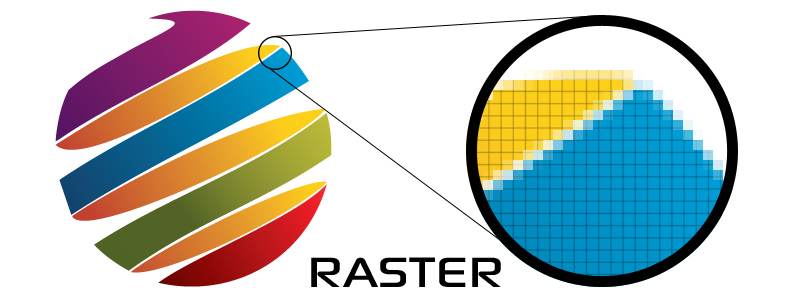
\includegraphics[width=\textwidth]{raster.jpg}
\caption{Zooming in on a Raster Graphics Image}
\end{figure}




Raster graphics are limited by the fact that the images it produces are resolution dependent. 
If you were to continuously zoom in on a raster image, eventually the image would suffer from image degradation, caused by making the small pixels in the original image visible.
Despite this problem, people use raster graphics because they are better at creating images not based on line art shapes. 
The pixel editing method of raster graphics makes it easier to use techniques such as subtle chromatic gradations, making forms with mathematically complicated or undefined lines and shapes, and complex composition. 
Pixel editing also makes creating different tools for raster graphics easier, since the makers can just define how pixels are effected based on where the user is working. 
\begin{figure}
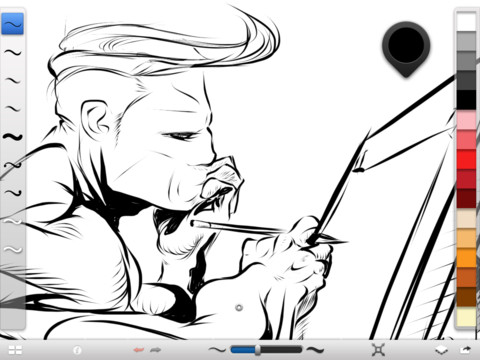
\includegraphics[width=\textwidth]{sketchbook.jpg}
\caption{Creating a Raster Image in Sketchbook}
\end{figure}



Examples of popular raster graphics software are Corel Painter, Adobe Photoshop, Microsoft's Paint.NET and MSPaint, the open-source GIMP software, and Autodesk's Sketchbook.

\pagebreak

\subsubsection{Vector Graphics}

Vector graphics is the representation of an image by the use of geometrical primitives such as points, lines, curves, shapes and polygons. 
Vector graphics are based on leading vectors though series of control points. Each of these points has a defined xy coordinate of the work space and determines the direction of the vector. 
Vectors can also be assigned a variety of properties such as its color, thickness, and fill. 

\subsubsection{Sketchbook Pro} http://www.autodesk.com/products/sketchbook-pro/features/all/gallery-view

Sketchbook Pro is a pixel drawing software application. It was originally made by Alias Systems Corporation, but is now owned and produced by Autodesk. Sketchbook is intended to simulate real-world art techniques such as pencil sketching, airbrushing, and painting. The work is saved as a bitmap where the color of each pixel in the image is stored. 

\subsubsection{Illustrator} http://www.adobe.com/products/illustrator.html

Illustrator is a vector graphics editor made by Adobe Software. It uses geometric primitives such as points, lines, curves, and polygons to create images, unlike raster programs that edit the individual pixels of an image. Illustrator is not an attempt to mimic real world art techniques; rather, it attempts to provide a new set of tools that allow for better editing and tuning of artwork only possible because of the systems mathematical representation of images. The current version, Illustrator CC, is the seventeenth edition of the product.

\subsubsection{Mischief} https://www.madewithmischief.com/

Mischief is another vector graphics editor created by Made With Mischief, now owned by The Foundry. Although it uses vector graphics, it does not allow for the precise editing of curves as seen in Illustrator. Instead it attempts to use vector graphics to simulate real world art techniques, like Sketchbook does. It features an infinite canvas for a free-form and dynamic sketching environment. This is allowed by using a data-structure called Adaptive Distance Fields, which allows them to greatly reduce the storage size of the vectors that the user creates at the cost of the ability to edit the vectors. This allows for incredibly detailed and large scale art withing the same file.


\subsection{3-D Modeling in CAD}

Rhino

AutoCAD

Maya / 3DMAX

Sketchup

\subsection{3-D Sketching in CAD}

Talk abouw how people have tried to bring 3-D sketching to computers

\subsubsection{CATIA Natural Sketch}

Natural Sketch is a feature inside of the CATIA modeling software by Dassault Systemes. Natural Sketch allows the user to draw on a virtual plane, a 3-D model, and the plane where the screen lies in the 3D environment. It features the abilities to alter the pen style, alter the number of control points used to make the post sketch curve, automatically change the camera view to align with the drawing plane if one is being used, copy and alter individual strokes, and generate models from the 3-D sketch.

\begin{figure}

\begin{subfigure}{\textwidth}
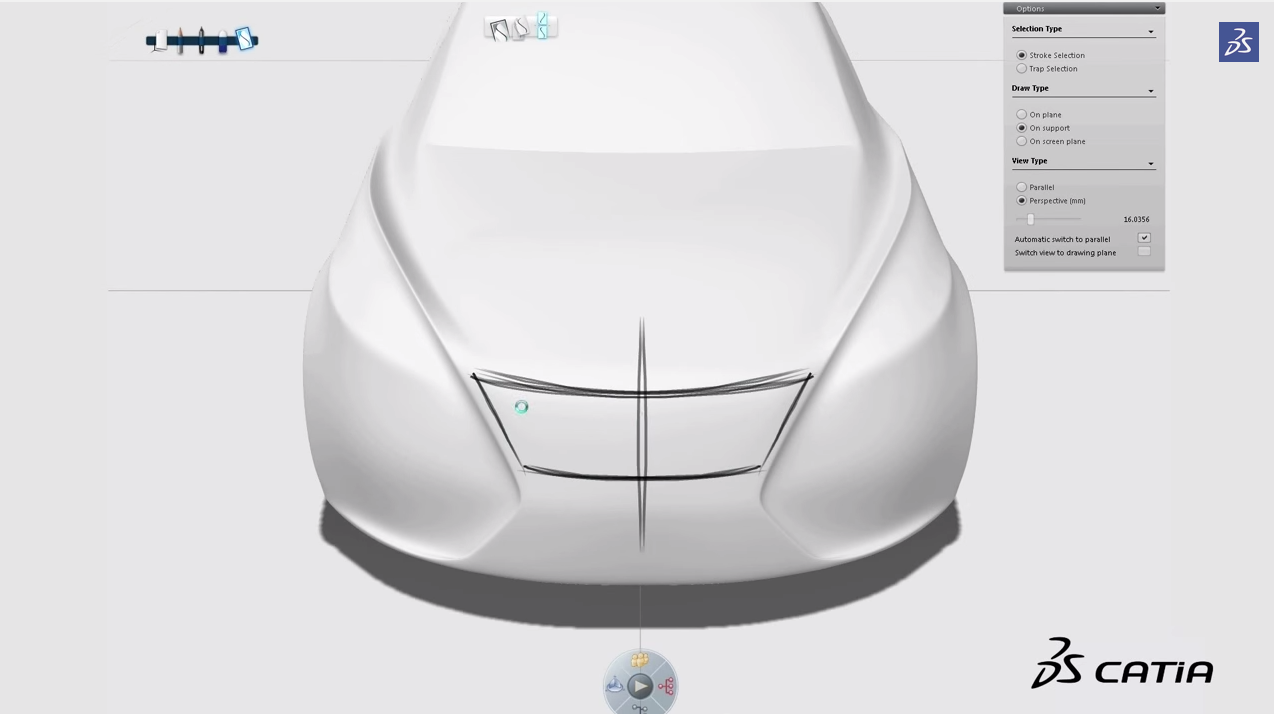
\includegraphics[width=\textwidth]{CATIA1}
\caption{Beginning the sketch}
\end{subfigure}
\begin{subfigure}{\textwidth}
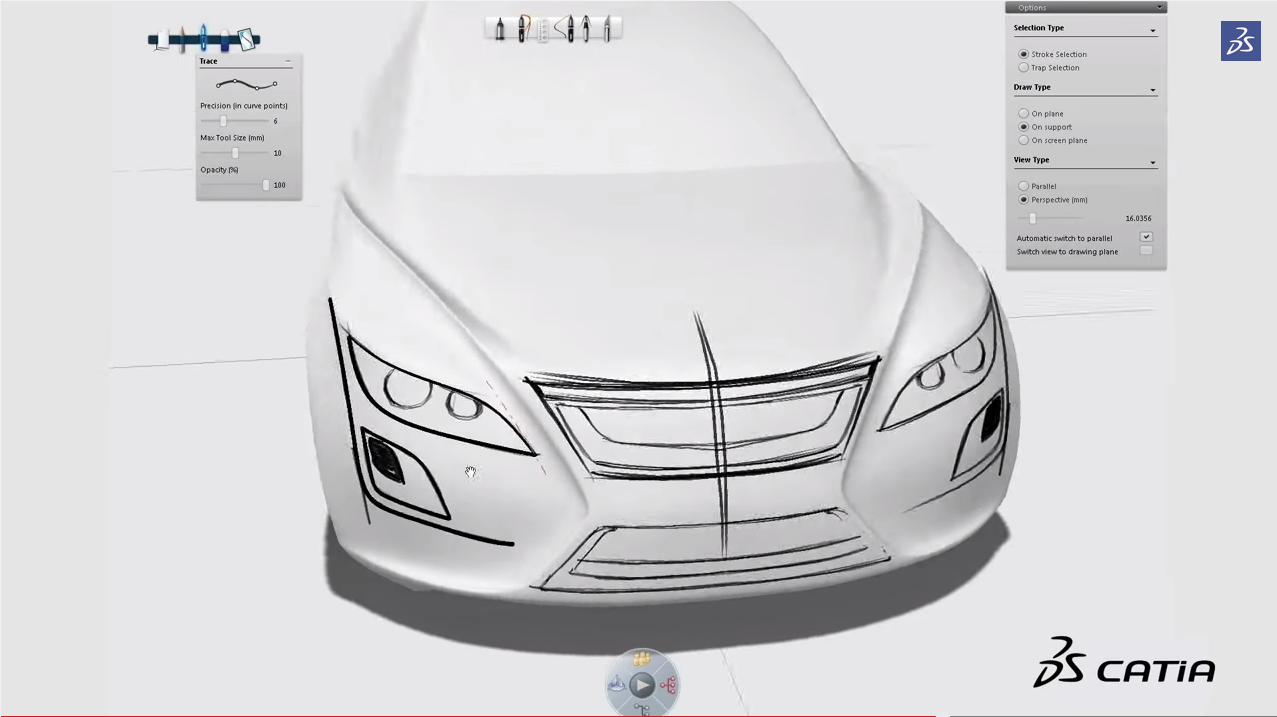
\includegraphics[width=\textwidth]{CATIA2}
\caption{Finishing the sketch}
\end{subfigure}

\caption{Using Natural Sketch to Add Detailing to a Car}
\end{figure}


\subsubsection{ILoveSketch / EverybodyLovesSketch}

EverybodyLovesSketch is a 3D curve sketching system from the University of Toronto's Dynamic Graphics Project Lab. It features a pen based gesture system, allowing the user to execute functions using rapid strokes, circles, and other defined gestures. Other features include dynamic sketch plane selection, single view definition of arbitrary extrusion vectors, multiple extruded surface sketching, copy-and-project of 3D curves, free-form surface sketching, and an interactive perspective grid. This project is based off of previous work by the same lab, ILoveSketch, which is the base 3D sketching functionality of the EverybodyLovesSketch project.

\subsubsection{Hyve 3D}

\begin{figure}

\begin{subfigure}{\textwidth}
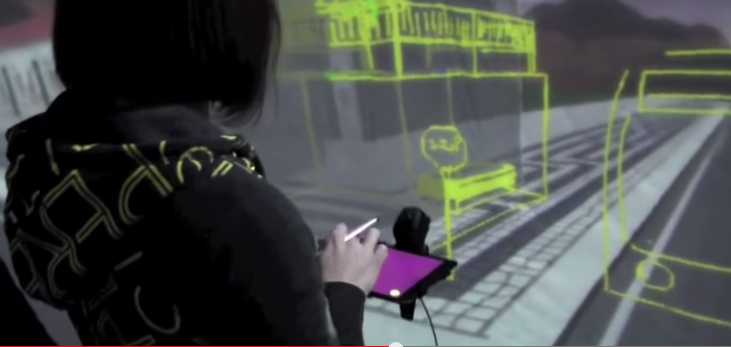
\includegraphics[width=0.9\linewidth]{Hyve3D1}
\caption{Using the tablet to draw}
\end{subfigure}
\begin{subfigure}{\textwidth}
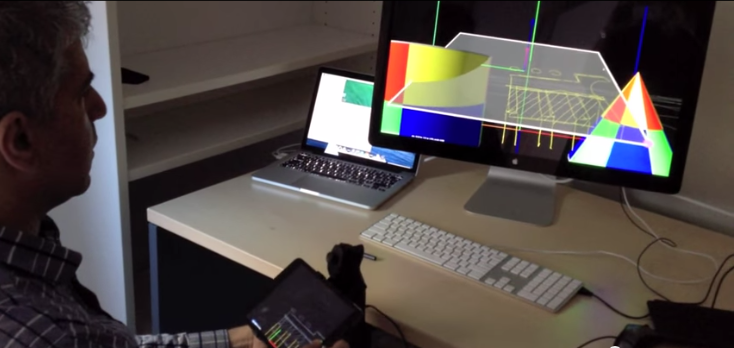
\includegraphics[width=0.9\linewidth]{Hyve3D2}
\caption{Manipulating the drawing plane}
\end{subfigure}

\caption{Examples of Hyve 3-D in use}
\end{figure}

Hyve 3D is an infinite virtual sketching environment from the University of Montreal. It uses two screens; a computer monitor to show the 3-D environment, and an iPad to draw. The sketching plane represented by the iPad is shown in the virtual environment, and is manipulated by moving and rotating the iPad in the real world. The user then pins the sketch plane in place and proceeds to draw at leisure. The advantage of this system is that it combines real world manipulation with virtual representation, eliminating the need for complex user interfaces and gestures. The disadvantage is that this kind of movement has no one-to-one feedback between the real world and the virtual, meaning that it is difficult to judge how your movements of the iPad effect the drawing place without confirming it visually.



\subsection{Other Work in 3-D Sketching}

Other forms of 3D content creation

Augmented Reality In-Situ 3D Sketching of Physical Objects $http://creativemachines.cornell.edu/papers/IUI09_Yee.pdf$

\subsubsection{Gravity} http://gravitysketch.com/

Gravity is an augmented reality 3D sketching tool using a tablet as the sketch base and a wearable screen to show the sketch. The tablet acts as a drawing plane, while the sketch can be moved via a set of controls on the tablet. The main idea is similar to Hyve 3D, in that you always draw in 2-D while you use your own sense of depth and position to understand what you are drawing, allowing for 3-D sketching without the use of perspective drawing. The difference is that this system allows you to use real world depth cues to augment your understanding of the virtual 3-D environment.

Sketch http://graphics.cs.brown.edu/research/sketch/

Polyes Q1 Pen http://technabob.com/blog/2014/12/29/polyes-q1-3d-sketching-pen/

\subsection{3-D Media Interaction}

Interacting with 3-D Media using modern input devices

Gestures vs. Postures: ‘Gestural’ Touch Interaction in 3D Environments 

\begin{verbatim}
$http://tobias.isenberg.cc/personal/papers/Isenberg_2012_GPG.pdf$
\end{verbatim}
A Survey of Interaction Techniques for Interactive 3D Environments http://www.grey-eminence.org/papers/EG2013-STAR.pdf

Interaction with 3-D environments using Multitouch Screens $http://www.researchgate.net/publication/236304194_Interaction_with_3D_Environments_using_Multi-Touch_Screens$

\pagebreak
\section{Input}

\begin{itemize}
\item Basic input chapter
\item Goal is to discuss where we are at in screen-based HCI
\item Hardware overview and methods, as well as gesture diagrams, use cases, etc
\end{itemize}
\subsection{Pen}

Discusses how people have attempted to solve HCI problems with pen input, as well as hardware and how the pen works 
Pen Based Interaction 
\begin{verbatim}
$http://www.academia.edu/2236260/Pen-based_Interaction_-_Next_Generation_User_Interfaces_WE-DINF-15756_$
\end{verbatim}
Pen-based User Interface 
\begin{verbatim}
$http://ieeexplore.ieee.org/stamp/stamp.jsp?tp=&arnumber=1349146$
\end{verbatim}
Experimental Analysis of Mode Switching Techniques in Pen-based User Interfaces http://research.microsoft.com/en-us/um/people/kenh/papers/p226-li.pdf
\subsection{Touch}

\subsection{Gesture}

\begin{figure}
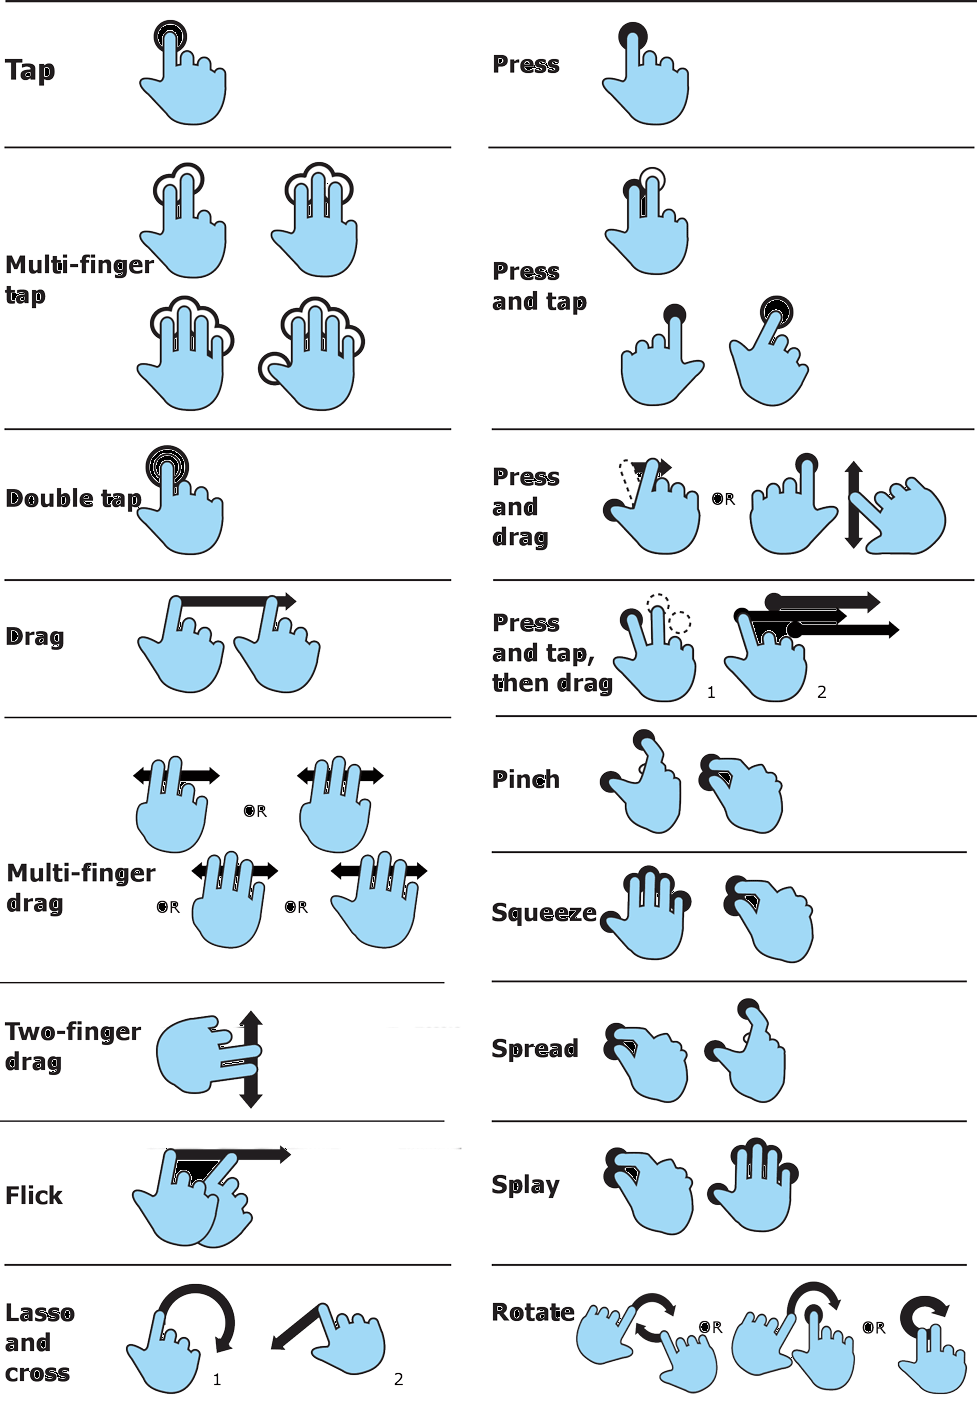
\includegraphics[width=0.9\linewidth]{GestureLibrary}
\caption{Touch Gesture Library}
\end{figure}
\begin{figure}
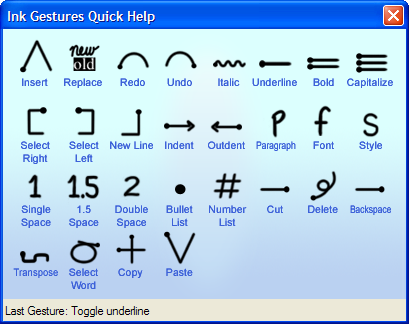
\includegraphics[width=0.9\linewidth]{pengestures}
\caption{Example Pen Gestures}
\end{figure}

\pagebreak

\section{Strokes, the Base of the Sketch}

\begin{itemize}
\item Spline talk chapter
\item Go over the inverse spline equation and the math behind the optimization
\item Get into 2-D to 3-D projection of strokes, and storage
\end{itemize}

\begin{figure}
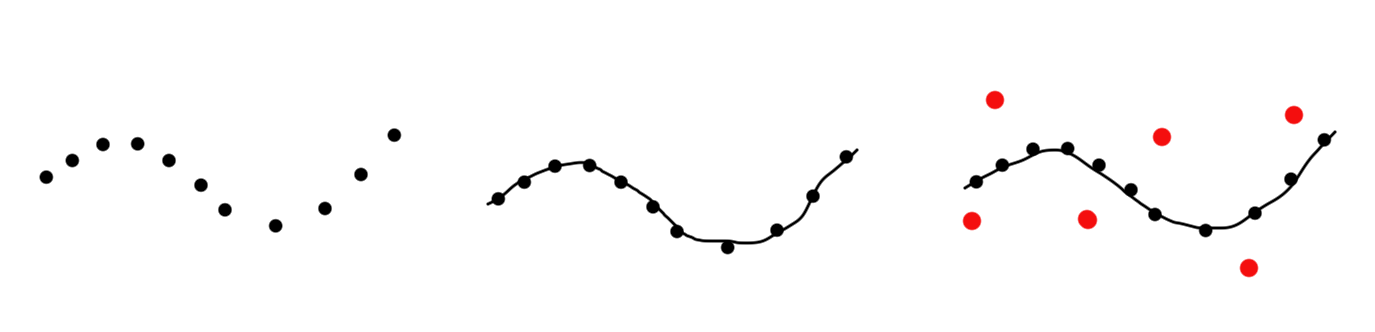
\includegraphics[width=0.9\linewidth]{CreatingACurve}
\caption{Rough Diagram of Optimizing a Curve using Control Points}
\end{figure}

Curve Global Interpolation http://www.cs.mtu.edu/~shene/COURSES/cs3621/NOTES/INT-APP/CURVE-INT-global.html

Smooth Spline Through Prescribed Points https://www.particleincell.com/2012/bezier-splines/

\subsection{Creating a Stroke}
\begin{itemize}
\item user inputs a series of points on the screen
\item storing all points too expensive, need to optimize
\item solution: create a curve based on the points that is defined by a smaller set of control points
\end{itemize}

\subsection{Definition of Splines}

Math goes here

\subsection{Inverse Spline Calculation}
Math goes here

\pagebreak
\section{Sketching in 3-D}

\begin{itemize}
\item Discuss how we get from the last chapter to 3-D sketching
\item Discuss Ray Casting and drawing surfaces
\item show system
\end{itemize}

\begin{figure}
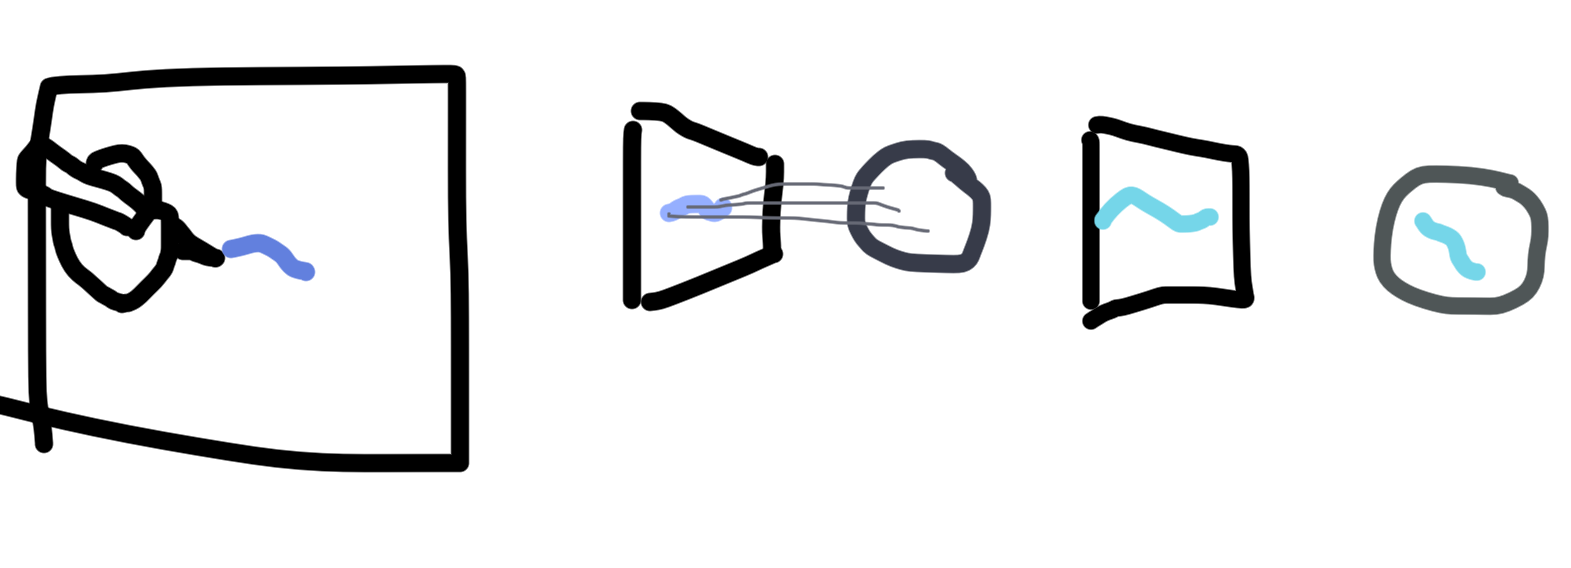
\includegraphics[width=0.9\linewidth]{StrokeProjection}
\caption{Rough Diagram of Projecting Stroke onto Drawing Surface}
\end{figure}

\subsection{Ray Casting}

\subsubsection{Acceleration Structure}
\begin{figure}[h]
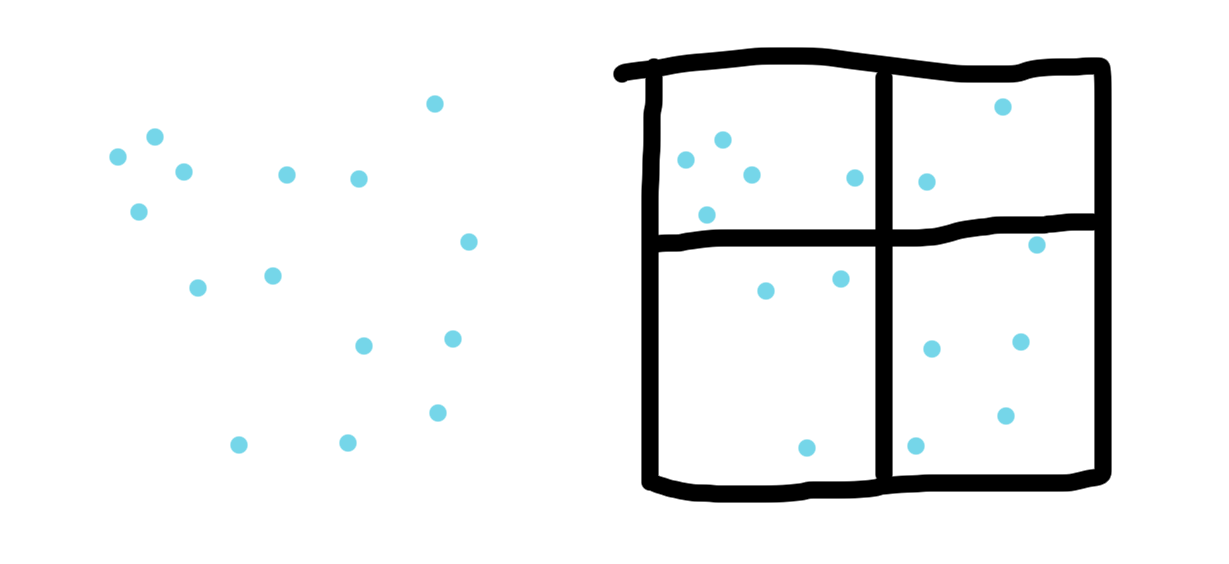
\includegraphics[width=0.9\linewidth]{AccelerationStructureExample}
\caption{Creating an Acceleration Structure}
\end{figure}
\subsubsection{Intersection}
Math goes here (Ray triangle intersection, Ray plane intersection, More in appendix? Reference?)
\subsection{Implementation}
\begin{itemize}
\item Display algorithm used
\item Discuss storage of strokes? (might not be particularly special)
\end{itemize}

\pagebreak
\section{Displaying Strokes}
Pen Styles section. This is getting complicated to the point that I think it needs it's own chapter
\begin{itemize}
\item Discuss reprojection of strokes into 2 space
\item Discuss pen styles and how pen styles are created (probably input reprojected 2D curve to geometry shader)
\item Discuss the what the actual styles are and the math behind them (possible appendix material after discussing one or two)
\end{itemize}
\pagebreak
\section{Usability and Feel: Bringing Physical Tools to the Virtual World}
\begin{itemize}
\item UX chapter
\item talk about how people actually use the system tools
\item talk about random quality of life features (page turning between layers, whatever else we come up with)
\end{itemize}
\subsection{Interacting with the 3D environment}
How do you move around the environment? How do you control things?
\subsection{Combining Pen and Touch}
Discus modality of system
\begin{figure}[h]
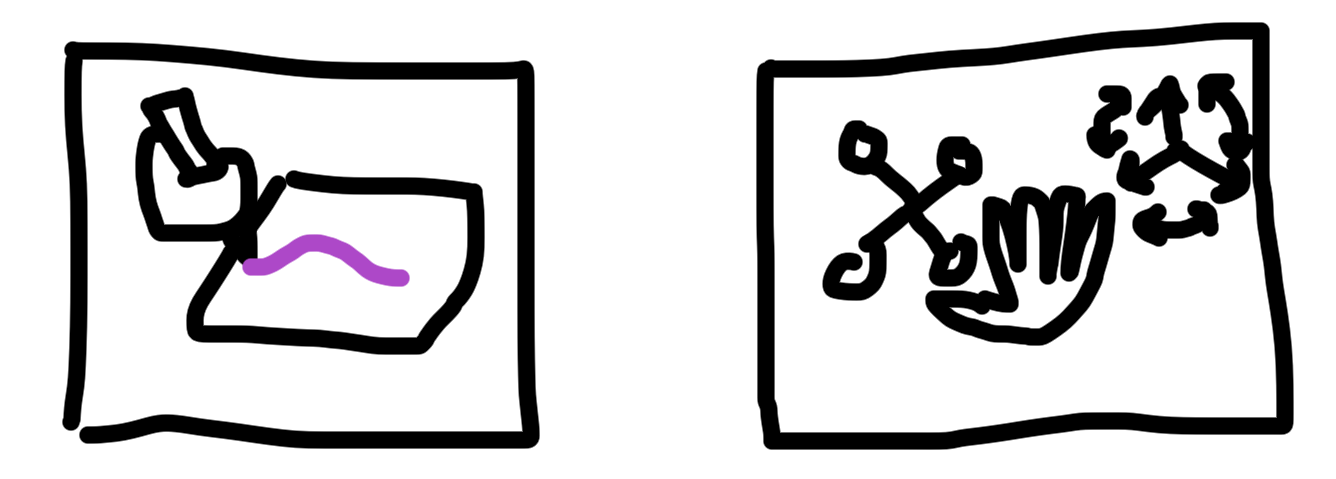
\includegraphics[width=0.9\linewidth]{Duality}
\caption{System Duality}
\end{figure}
\subsection{Turning the Page}
\begin{figure}[h]
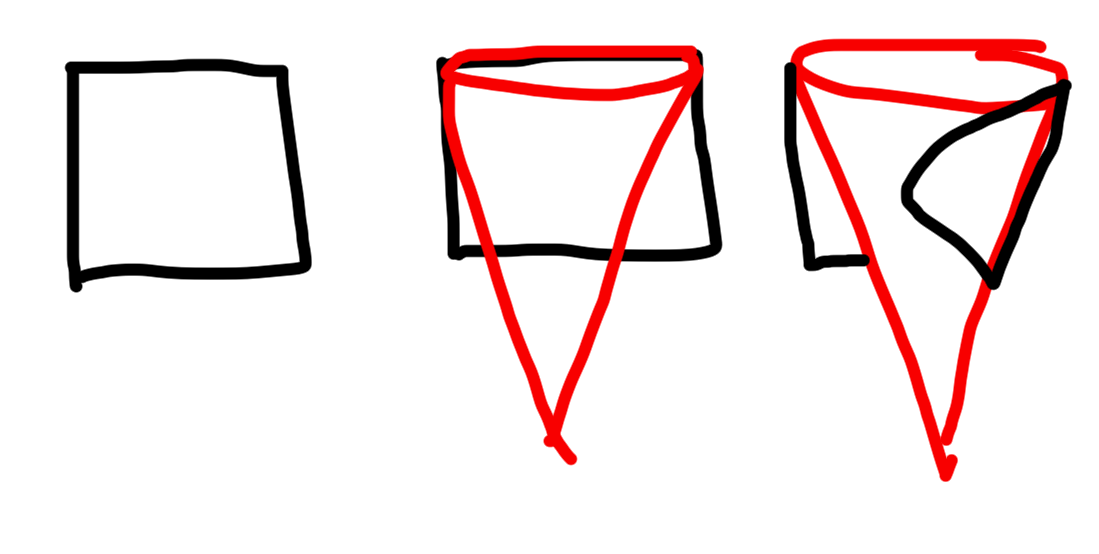
\includegraphics[width=0.9\linewidth]{TurningThePage}
\caption{Rough Diagram of math behind page turn}
\end{figure}
\begin{itemize}
\item Add reference to paper
\item show math
\end{itemize}


\pagebreak

\section{Conclusion}
Summary of everything goes here. More images of the system in use and example use cases.
\end{document}